\chapter{Proposta}
\label{cap4}

O algoritmo descrito no capítulo anterior possui várias possibilidades de ganho de desempenho. Todavia, para que isso seja possível, uma versão em C/C++ precisará ser desenvolvida.

Este trabalho de conclusão de curso possui três etapas principais. Na primeira etapa, será feita uma implementação em C++ do algoritmo de cripto-compressão \gmpr. Com base nesta solução proposta, na segunda etapa serão estudadas formas de paralelizar o código para obter-se um desempenho ainda melhor. As \apis \openMP, \mpi e/ou \cuda serão exploradas para implementar soluções paralelas e/ou distribuídas para este problema. Por fim, na terceira etapa, serão realizados experimentos para medir o desempenho das soluções paralelas propostas.

No presente momento, somente as etapas de cifragem/decifragem foram implementadas em C++. As etapas de compressão/descompressão serão implementadas ao longo do primeiro semestre de 2018. A versão atual do código em C++ está disponível no GitHub\footnote{\url{https://github.com/leandroperin/ParallelCryptoCompression}}.

A seguir, serão apresentadas algumas ideias iniciais de paralelização das etapas de cifragem/decifragem.

\section{Paralelismo com Multiprocessadores}

A primeira ideia de paralelização do código é a utilização do \openMP para executar as partes mais pesadas da aplicação em múltiplos núcleos do processador. Conforme visto no Capítulo~\ref{cap3}, o algoritmo possui muitos laços do tipo \texttt{for}, o que permite a utilização da biblioteca \openMP para executar esses laços em paralelo (através da diretiva \texttt{omp parallel for}), garantindo a correta execução das operações, porém em menos tempo.

Para isso, o objetivo inicial será definir em quais partes do código o programa leva mais tempo para executar, analisar se é possível quebrar essa parte em pedaços pequenos e atribuir múltiplas \texttt{threads} para a execução. Para isso, alguns experimentos preliminares foram feitos utilizando-se a ferramenta \texttt{Valgrind}\footnote{\url{http://valgrind.org/}} no Linux. A Figura~\ref{fig:valenc} apresenta os resultados obtidos para o algoritmo de codificação, enquanto a Figura~\ref{fig:valdec} apresenta os resultados para a decodificação.

\begin{figure}[t]
    \centering
    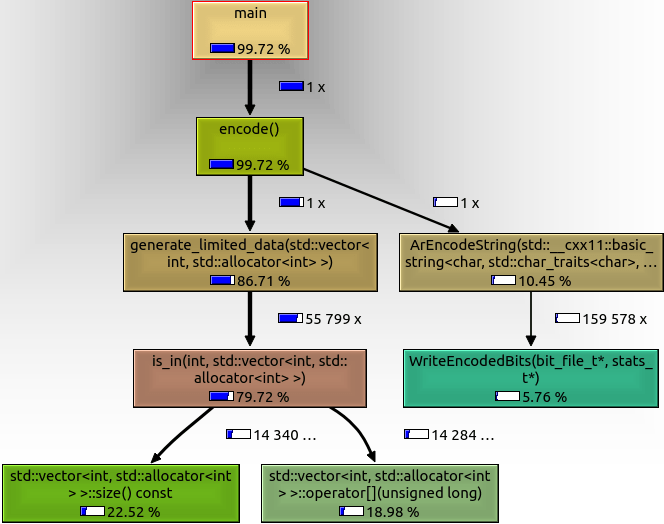
\includegraphics[width=8cm, height=6cm]{Images/ValgrindEncode.png}
    \caption{Resultados do Valgrind para a Codificação.}
    \label{fig:valenc}
\end{figure}

\begin{figure}[t]
    \centering
    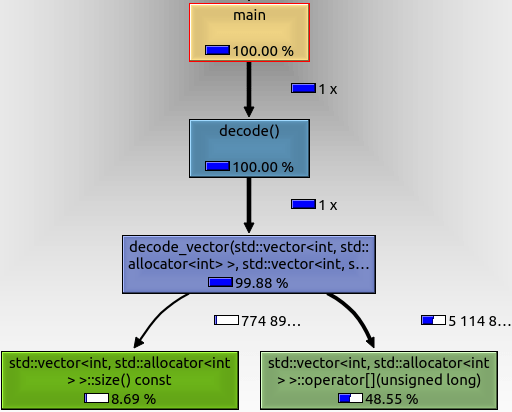
\includegraphics[width=8cm, height=6cm]{Images/ValgrindDecode.png}
    \caption{Resultados do Valgrind para a Decodificação.}
    \label{fig:valdec}
\end{figure}

Como é possível observar nas Figuras~\ref{fig:valenc} e~\ref{fig:valdec}, os métodos mais custosos em termos de tempo de execução são o \texttt{generate\_limited\_data()} para a parte de codificação, o qual utiliza o método \texttt{is\_in()} para verificar se algum caractere está presente na lista única de caracteres, e o \texttt{decode\_vector()} para a parte de decodificação, o qual usa o operador \texttt{[]} para acessar os elementos do vetor que contém os dados codificados.

O próximo passo é então fazer uso de regiões paralelas para dividir a computação executada nos métodos anteriormente citados a fim de melhorar o desempenho geral da solução. Após a definição das regiões paralelas, será necessário analisar se existem variáveis que serão compartilhadas entre as \textit{threads} e se há dependência entre elas. As cláusulas \texttt{shared} e \texttt{private} permitem descrever quais variáveis são compartilhadas entre todas as \textit{threads} e quais são privadas em cada \textit{thread}, respectivamente. Também, será verificada a existência de condições de corrida no código paralelizado. Nesses casos, regiões críticas do código, que são regiões que só podem ser executadas em uma \textit{thread} de cada vez, deverão ser protegidas com o uso da diretiva \texttt{omp critical}.

Por fim, será avaliada a possibilidade de uma solução híbrida com uso de \openMP e \mpi. Esta solução permitiria a execução da versão paralela da aplicação em \texttt{clusters}.

\section{Paralelismo com Aceleradores}

Tendo em  vista os resultados dos experimentos iniciais mostrados nas Figuras~\ref{fig:valenc} e~\ref{fig:valdec}, uma possibilidade seria a implementação de \textit{kernels} \cuda ou \opencl, uma solução de código aberto, para realizar a computação dos métodos mais custosos em \gpu. Neste caso, como mostrado no exemplo da Figura~\ref{fig:lstcuda}, será necessário implementar os \textit{kernels}, alocar memória na \gpu, copiar os dados que estão na \cpu e, por fim, liberar a memória utilizada.

As \gpus trabalham muito bem com operações matriciais, portanto uma possibilidade de melhora do código seria armazenar o conteúdo em matrizes e executar o algoritmo de cripto-compressão diretamente nas placas gráficas, garantindo um ganho de desempenho. \gpus possuem centenas de núcleos, e essa arquitetura massivamente paralela pode fazer o algoritmo \gmpr executar em um tempo consideravelmente menor.

Conteúdos que ganhariam bastante com o uso de \gpus são imagens e vídeos, afinal já são naturalmente armazenados em forma de matriz. A utilização do \cuda ou do \opencl seria bastante eficaz para esse tipo de conteúdo.

\section{Testes de Desempenho}

Após a implementação das soluções propostas (\openMP, \mpi e/ou \cuda/\opencl) serão feitos inúmeros testes e medições de desempenho, para que seja descoberta a melhor e mais rápida maneira de executar o algoritmo, garantindo o menor tempo de execução possível.